\FloatBarrier
\section{Генератор Колпитца} % _COLP_

\LinkRef{
  colp: ASAU-21, APIR-2013
}

В ряде радиоэлектронных устройств используются
генераторы сигналов, способные генерировать разнообразные виды  сигналов, в том числе
сложно-периодические и хаотические.
В частности, генератор  Колпитца~\cite{kennedy_chaos_colpitts,atu_asau21}, который, в
зависимости от условий,   может
генерировать  колебания,  как  близкие  к  гармоническим,  так  и  проявлять
хаотическую  динамику  в  широком  спектральном   диапазоне.   Идентификация
параметров рассматриваемого генератора  необходима,  с  одной  стороны,  для
обеспечения  требуемых  режимов  работы.  С  другой  стороны,  информация  о
параметрах системы необходима при проведении  контроля  работоспособности  в
процессе эксплуатации устройства~\cite{atu_apir2013}.

На рис.~\ref{atu:f:colp_schem} приставлена одна из электрических схем,
реализующих генератор Колпитца на биполярном транзисторе.
Из множества схем, данная была выбрана из-за наличия
одного источника напряжения и простоты схемотехнической реализации генератора.


\begin{figure}[htb!]
\begin{center}
% vi:syntax=tex

\begin{circuitikz}[line width=0.7]
  \ctikzset{bipoles/thickness=2}
  \def\Top{8.0}
  %
  \draw (3.0,3.0) node[npn](npn) {};
  \draw (2.8,3.0) circle[radius=0.5];
  %\draw (npn.center) circle[radius=0.5];
  %
  \draw (0.0,0.0)
   to[R,l=$R_2$,-*]  (0.0,3.0)
   to[R,l=$R_1$]     (0.0,\Top)
   to[short]         (6.0,\Top)
   to[battery,l=$V_{cc}$] (6.0,0.0)
   -- (0.0,0.0);
  %
  \draw (1.5,0.0) to[C,l=$C_0$,*-*] (1.5,3.0);
  \draw (0.0,3.0) -- (npn.base);
  \draw (3.0,0.0) to[vR,l=$R_e$,*-*] (3.0,2.0)
   to[short] (npn.emitter);
  \draw (npn.collector)
   to[L,l=$L$,i<=$I_L$] (3.0,6.0)
   to[R,l=$R_c$] (3.0,\Top);
  %
  \draw (4.5,0.0) to[C,l=$C_2$,v=$V_2$,*-*] (4.5,2.0);
  \draw (4.5,2.0) -- (3.0,2.0);
  \draw (4.5,2.0) to[C,l=$C_1$,v=$V_1$]     (4.5,4.0);
  \draw (4.5,4.0) -- (3.0,4.0);
  \filldraw (3.0,4.0) circle[radius=0.05];
\end{circuitikz}



%\begin{tikzpicture}[circuit ee IEC,very thick,circuit symbol unit=2.5mm]
%%\tikzset{circuit declare symbol=transistor}
%%\tikzset{set transistor graphic=transistor IEC graphic}
%  \node (R2)    at (0.0,0.0) [elelem,point up,resistor={info = $R_2$}] {};
%  \node (pR1R2) at (0.0,1.5) [contact] {};
%  \node (R1)    at (0.0,3.0) [elelem,point up,resistor={info = $R_1$}] {};
%  %
%  \node (C0)    at (1.5,0.0) [point up,elelem,capacitor={info = $C_0$}] {};
%  \node (pR2C0) at (1.5,1.5) [contact] {};
%  %
%  \node (Re)    at (3.0,0.0) [elelem,point up,resistor={adjustable,info = $R_e$}] {};
%  %\node (Q1)    at (3.0,1.5) [elelem,point right,transistor] {};
%  \node (L)     at (3.0,3.0) [elelem,point up,inductor={info = $L$}] {};
%  \node (Rc)    at (3.0,4.5) [elelem,point up,resistor={info = $R_c$}] {};
%  %
%  \node (C2)    at (4.5,0.0) [point up,elelem,capacitor={info = $C_2$}] {};
%  \node (C1)    at (4.5,3.0) [point up,elelem,capacitor={info = $C_1$}] {};
%  %
%  \node (Bat)   at (6.0,0.0) [point up,elelem,battery={info = $Vcc$}] {};
%\end{tikzpicture}


\end{center}
\caption{Электрическая схема генератора Колпитца на биполярном транзисторе}
\label{atu:f:colp_schem}
\end{figure}

При создании модели генератора Колпитца систему уравнений можно
заранее упростить, если заметить, что
делитель на резисторах
$\mathrm{R}_1$, $\mathrm{R}_2$,
вместе с конденсатором
$\mathrm{C}_0$ обеспечивают
постоянство потенциала базы
$V_b = V_{CC} \frac{R_1}{R_1+R_2}$,
поэтому из дальнейшего рассмотрения данные элементы следует
исключить.

Рассмотрев процессы заряда конденсаторов и изменение тока через
катушку индуктивности, получим следующую систему уравнений:
%
\begin{equation}
\label{atu:eq:colp_phys}
\begin{dcases}
  C_1 \od{V_{1}}{t}  = I_L - I_{CE} , \\
  L\, \od{I_L}{t} \; = V_{CC} - V_{1} - V_{2} - I_L R_C , \\
  C_2 \od{V_{2}}{t}  = I_L - \frac{V_{2}}{R_e}.
\end{dcases}
\end{equation}
%
%
%\noindent
где
$V_{CC} $ -- напряжение питания,
$V_1,$ $V_2$ -- разность потенциалов между выводами конденсаторов
$\mathrm{C}_1$ и $\mathrm{C}_2$ соответственно,
$I_L$, $I_{CE}$ -- токи катушки индуктивности и транзистора (коллектор-эмиттер).

Перейдём к безразмерным величинам.
При переходе к безразмерному виду следует определить,
какие физические параметры определяют безразмерные величины.
Это потребуется для синтеза критерия идентификации.
Для упрощения рассмотрения, не снижая общности,
будем считать $C_1 = C_2 = C$.

Прежде всего, воспользуемся тем, что система содержит только один
активный нелинейный компонент -- транзистор.
Следовательно, именно этот элемент определяет
масштаб по напряжению. В простейшей модели транзистора
такой масштабной величиной может служить
$V_{je}$ -- падение напряжения на переходе база-эмиттер
в активном режиме. Следовательно, все разности потенциалов в схеме можно нормировать
на эту величину.

Динамические свойства (в т.ч. условия начала генерации и перехода в хаотический режим) определяются
соотношением активных и реактивных свойств системы. При этом величина
$ \rho = \sqrt{L/C} $ имеет размерность сопротивления
и определяет величину реактивного сопротивления. Эту величину можно использовать
для обезразмеривания активных сопротивлений.

Для приведения токов к безразмерному виду, с учётом уже выбранных величин,
следует использовать величину $ V_{je} / \rho$.


Исходя из всего вышеперечисленного, обозначим:
%
\[
  x = \frac{V_{1}}{V_{je}} ; \quad
  y = \frac{\rho I_L}{V_{je}} ; \quad
  z = \frac{V_{2}}{V_{je}}, \quad
  i_{ce} = \frac{\rho I_{ce}}{V_{je}}, \quad
  c = \frac{V_{CC}}{V_{je}}, \quad
  e = \frac{V_{b}}{V_{je}}.
\]
%
\[
  b = \frac{R_c}{\rho}; \quad
  d = \frac{\rho}{R_e}. % sic!
\]

Система уравнений принимает вид:
%
\begin{equation}
\label{atu:eq:colp_phys2}
\begin{dcases}
  \od{x}{t}  = \dfrac{1}{\rho C}  y - \dfrac{1}{\rho C} i_{ce} , \\
  \od{y}{t}  = \dfrac{\rho}{L} c    - \dfrac{\rho}{L} r_c y - \dfrac{\rho}{L} x- \dfrac{\rho}{L} z, \\
  \od{z}{t}  = \dfrac{1}{\rho C}  y - \dfrac{1}{\rho C} \dfrac{1}{r_e} z.
\end{dcases}
\end{equation}

Общий множитель $ \frac{1}{\rho C} = \frac{\rho}{L} = \sqrt{\frac{1}{LC}} $ в правых частях уравнений
естественным образом задаёт масштаб по времени.
Это подчёркивает, что частотные характеристики рассматриваемого генератора,
в отличие, например, от релаксационного,
определяются ёмкостью и индуктивностью,
поэтому масштаб времени задаём так:
$ T_s = \sqrt{L C} $.
Тогда безразмерное время $t_s$
и соответствующие производные
будут определяться как:
%
\[
  t_s = \frac{t}{T_s}; \quad
  \mathrm{d}\, t = T_s \mathrm{d}\, t_s; \quad
  \od{}{t}  = \frac{1}{T_s} \od{}{t_s}; \quad
  \od{x}{t_s} \equiv \dot{x} = T_s \od{x}{t} .
\]

Поведение величины $I_{ce}$ (в дальнейшем просто $I_c$) достаточно хорошо описывает модель
Эберса-Молла~\cite{horowitz}:
%
\begin{equation}
  I_c = I_s \left( \exp\frac{V_{be}}U_t{} - 1 \right),
  \label{atu:eq:ebers-moll}
\end{equation}
%
%\noindent
где
$I_s$ -- ток насыщения (паспортная или определяемая экспериментально величина),
$U_t=kT/q$,
$q = \SI{1.6e-19}{\coulomb}$ -- заряд электрона,
$k = \SI{1.38e-23}{\joule/\kelvin}$ -- постоянная Больцмана.
Необходимо учесть, что в режиме отсечки ($V_b < V_e$) ток коллектора пренебрежимо мал,
а в режиме насыщения определяется другими элементами схемы.
Существуют и более сложные модели, например,
программы для моделирования электронных схем часто используют так называемую SPICE модель.

К сожалению, при моделировании генератора Колпитца в литературе,
посвящённой хаотической динамике, используют
простейшую модель транзистора, считая, что переход
база-эмиттер открывается при $V_{BE} = V_{je}$, $ I_c \gg I_b$,
а ток коллектора
%
\begin{equation}
I_c =
  \begin{cases}
    \alpha ( V_b - V_e - V_{je} ), & V_b - V_e > V_{je} \\
    0                              & \text{otherwise}.
  \end{cases}
  \label{atu:eq:bjt_libear_model}
\end{equation}



С учётом всего вышеизложенного получаем следующую систему уравнений:
%
\begin{equation}
\label{atu:eq:colp}
\begin{cases}
  \dot{x} = y - a F(z), \\
  \dot{y} = c - x - by - z, \\
  \dot{z} = y - d z.
\end{cases}
\end{equation}

При этом параметр $b$ характеризует соотношение
активного и реактивного сопротивления,
и, следовательно, режима работы генератора.
Величиной этого параметра проще всего управлять,
изменяя $R_c$.
Ставится задача идентификации данного параметра.

При физическом моделировании, проведённом в рамках данной работы использовались следующие
элементы с соответствующими параметрами:
%
\[
  V_{cc} = \SI{12.06}{\volt},          \;
  R_1 = R_2 = \SI{2.2}{\kilo\ohm},     \;
  R_e = \SI{430}{\ohm},
\]
%
\[
  C_1 = C_2 = \SI{1.03}{\micro\farad}, \;
  L = \SI{6.22}{\milli\henry},         \;
  T = \SI{305}{\kelvin},
\]
%
\[
  \text{Q: 2N2222A}, \quad
  h_{fe}=285, \;
  V_f = \SI{0.677}{\volt}, \;
  I_s = \SI{9.61e-14}{\ampere}, \;
  \alpha \approx 1.
\]

Тогда безразмерные коэффициенты:
\[
 a = 77,     \quad
 c = 18.08,  \quad
 d = 0.19,   \quad
 e = 9.07.
\]
%
\[
F(z) =
\begin{cases}{l}
  e-1-z, & z \le e-1  \\
  0,     & z  >  e-1
\end{cases}.
\]


Диапазон изменения идентифицируемого параметра
$b \in [ 0.02; 4.2 ]$
определяется, с одной стороны, собственным сопротивлением катушки индуктивности,
с другой -- срывом генерации.


На рис.~\ref{atu:f:colp_real_xzz}--\ref{atu:f:colp_model_f} предствлены как результаты реального эксперимента,
так и данные, полученные в результате численного моделирования динамики системы (\ref{atu:eq:colp}).
Представлены проекции аттракторов на плоскость $(x+z,z)$ (естественный вид для оциллографа),
трёхмерный вид аттракторов, и спектры.
На каждом рисунке представлено три режима: обычный, момент первого удвоения периода и хаотический режим.


\begin{figure}[htb!]
 \centerline{
   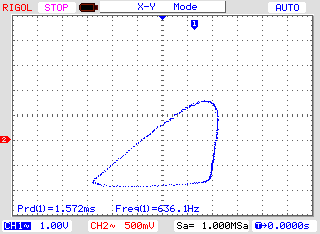
\includegraphics[width=0.32\textwidth]{p/cha/colp/colp_m1_vv.png}
   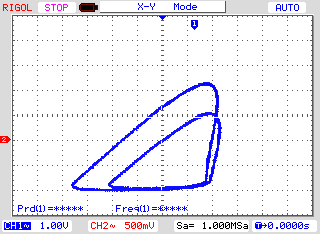
\includegraphics[width=0.32\textwidth]{p/cha/colp/colp_m2_vv.png}
   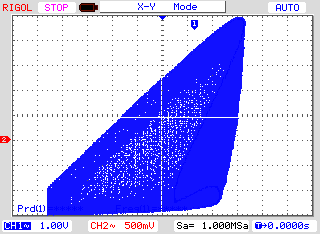
\includegraphics[width=0.32\textwidth]{p/cha/colp/colp_m3_vv_ac.png}
 }
  \caption{Проекции аттракторов реальной системы Колпитца на плоскость $(x+z,z)$
  для трёх режимов}
  \label{atu:f:colp_real_xzz}
\end{figure}

\begin{figure}[htb!]
 \centerline{
   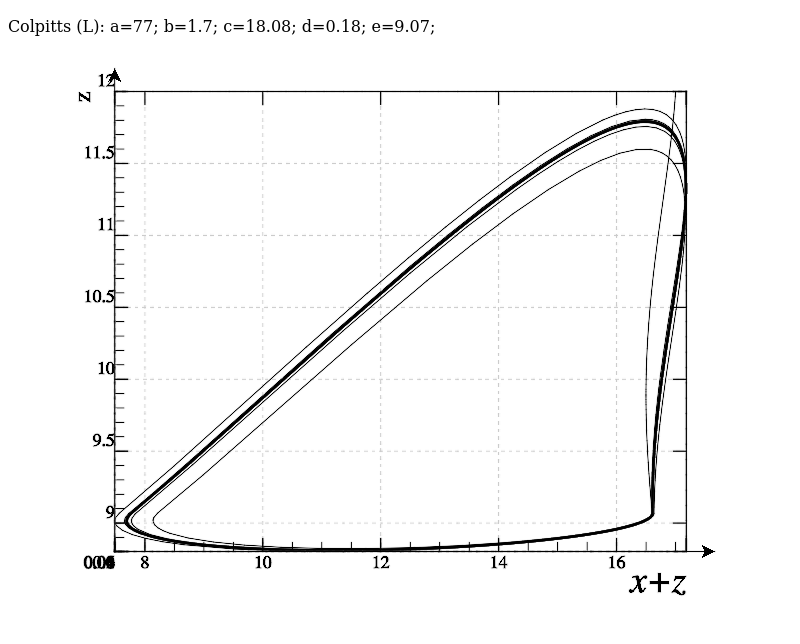
\includegraphics[width=0.32\textwidth]{p/cha/colp/colp_0-p_z_xpz_b=1x70.png}
   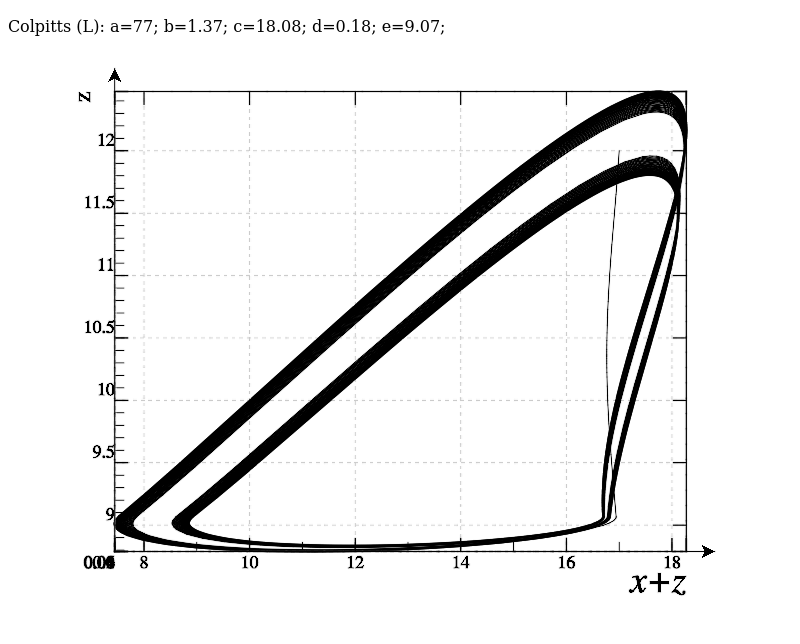
\includegraphics[width=0.32\textwidth]{p/cha/colp/colp_0-p_z_xpz_b=1x37.png}
   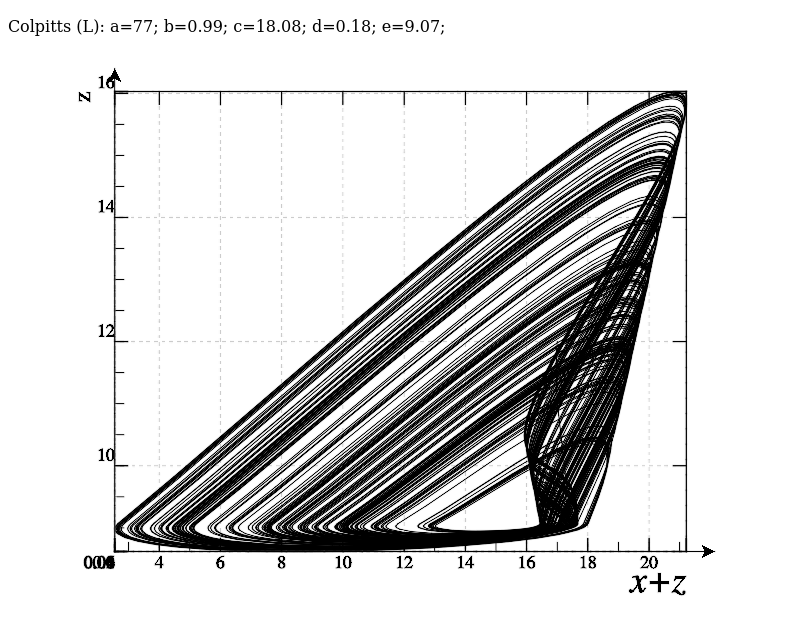
\includegraphics[width=0.32\textwidth]{p/cha/colp/colp_0-p_z_xpz_b=0x99.png}
 }
  \caption{Проекции аттракторов модели (\ref{atu:eq:colp}) системы Колпитца на плоскость $(x+z,z)$
  для трёх режимов}
  \label{atu:f:colp_model_xzz}
\end{figure}


\begin{figure}[htb!]
 \centerline{
   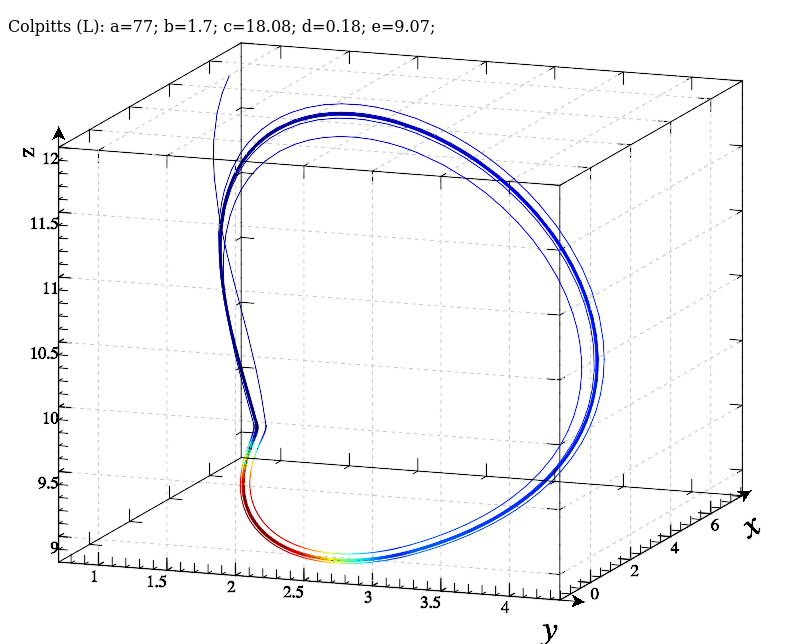
\includegraphics[width=0.32\textwidth]{p/cha/colp/colp_0-p_xyz_b=1x70.png}
   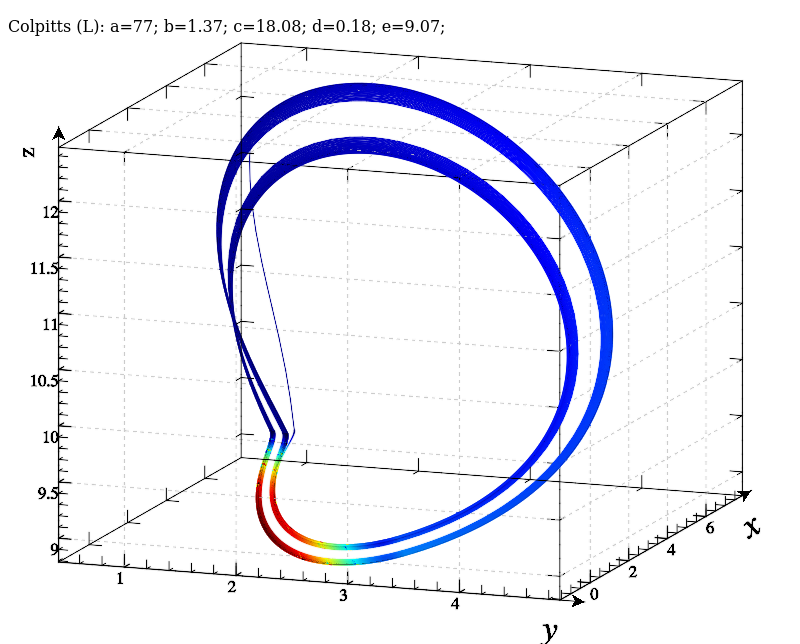
\includegraphics[width=0.32\textwidth]{p/cha/colp/colp_0-p_xyz_b=1x37.png}
   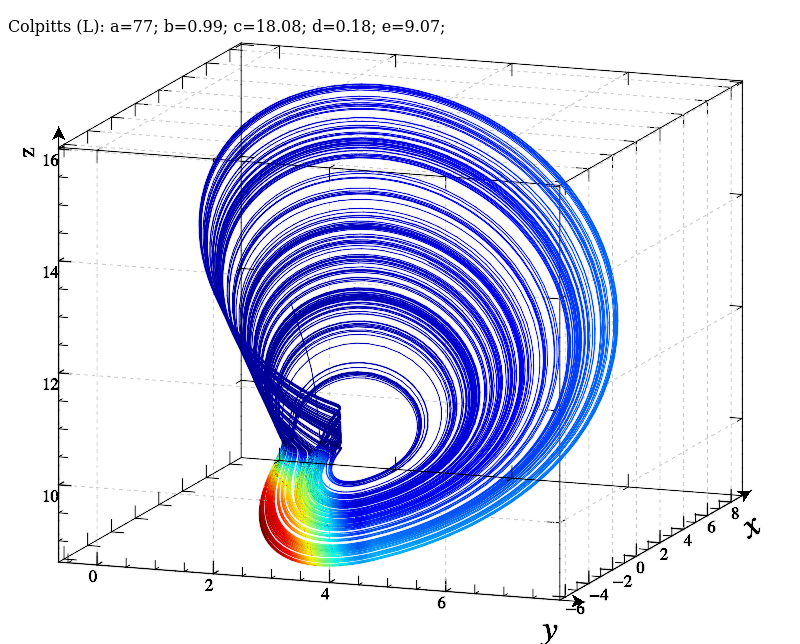
\includegraphics[width=0.32\textwidth]{p/cha/colp/colp_0-p_xyz_b=0x99.png}
 }
  \caption{Аттрактороы модели (\ref{atu:eq:colp}) системы Колпитца для трёх режимов}
  \label{atu:f:colp_model_xyz}
\end{figure}

\begin{figure}[htb!]
 \centerline{
   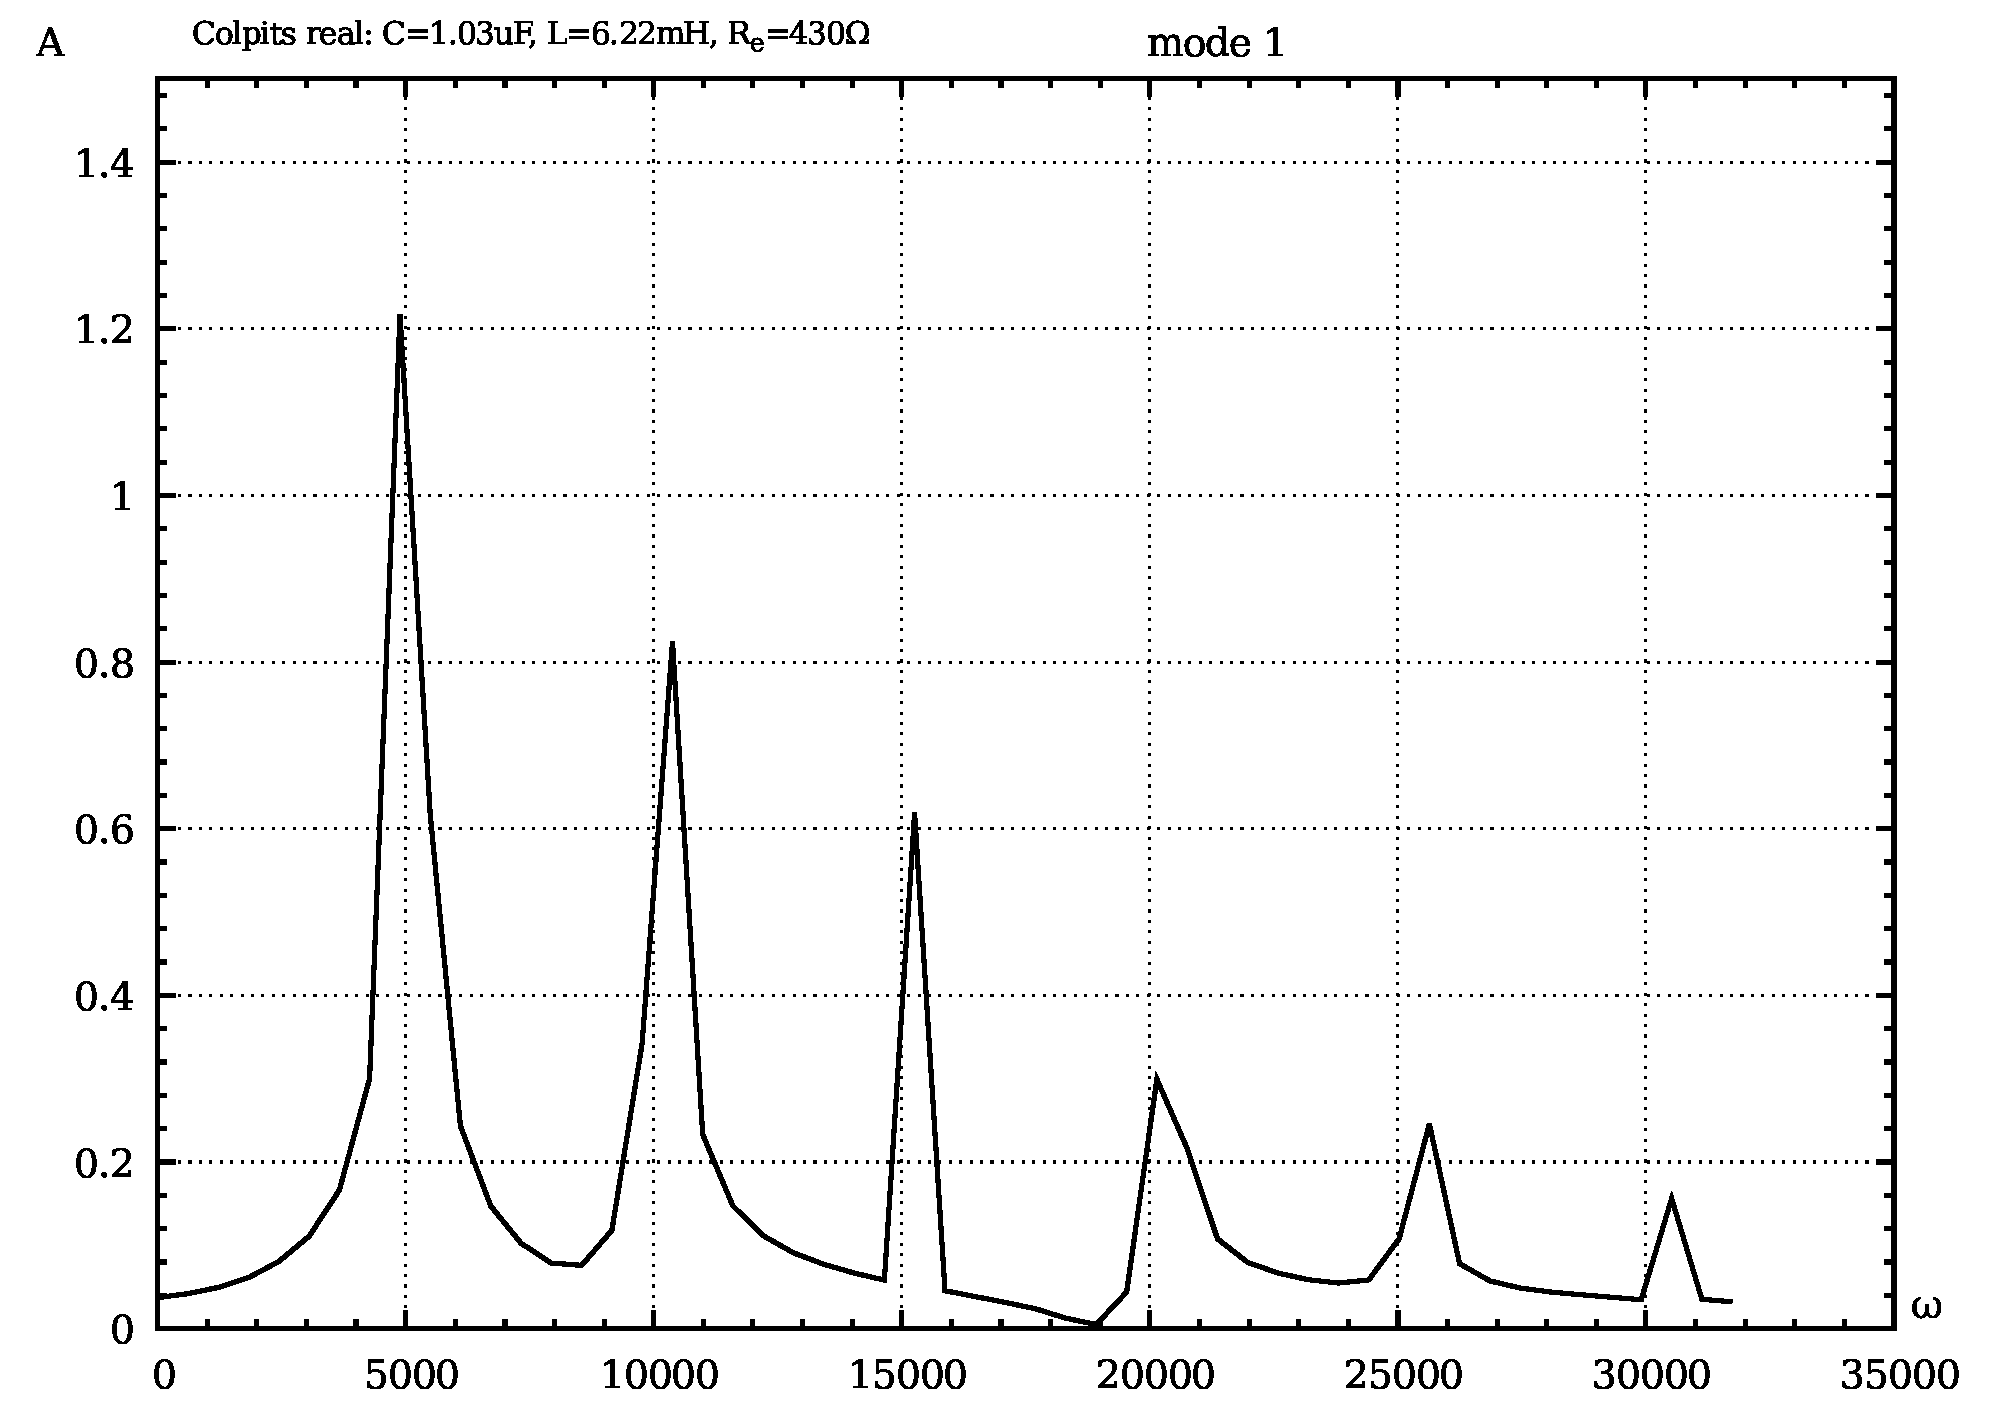
\includegraphics[width=0.32\textwidth]{p/cha/colp/colp_m1_f.png}
   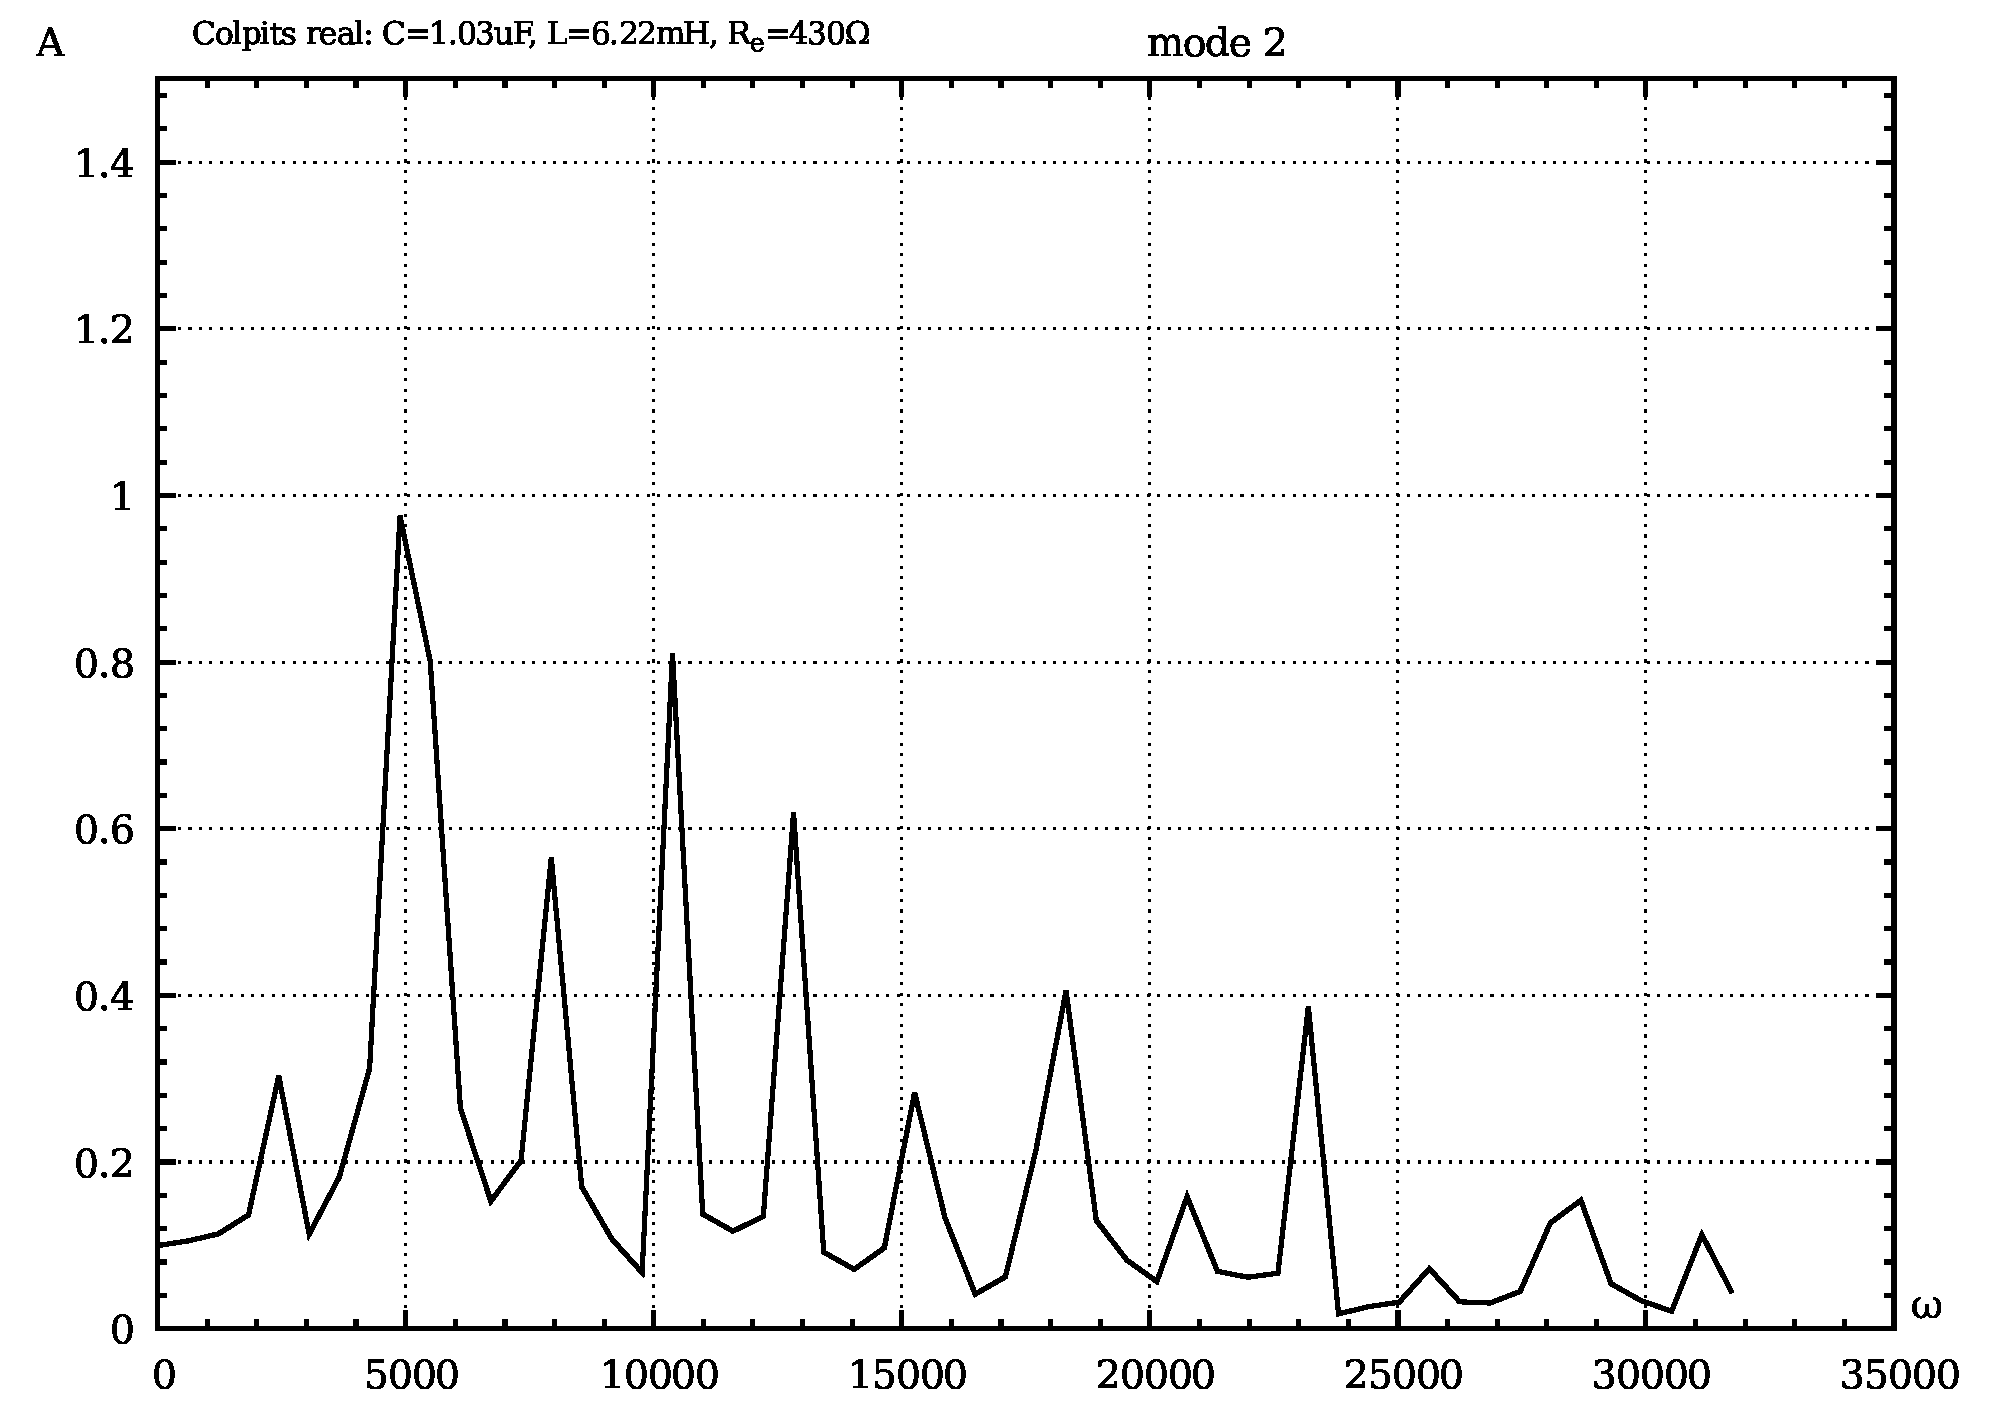
\includegraphics[width=0.32\textwidth]{p/cha/colp/colp_m2_f.png}
   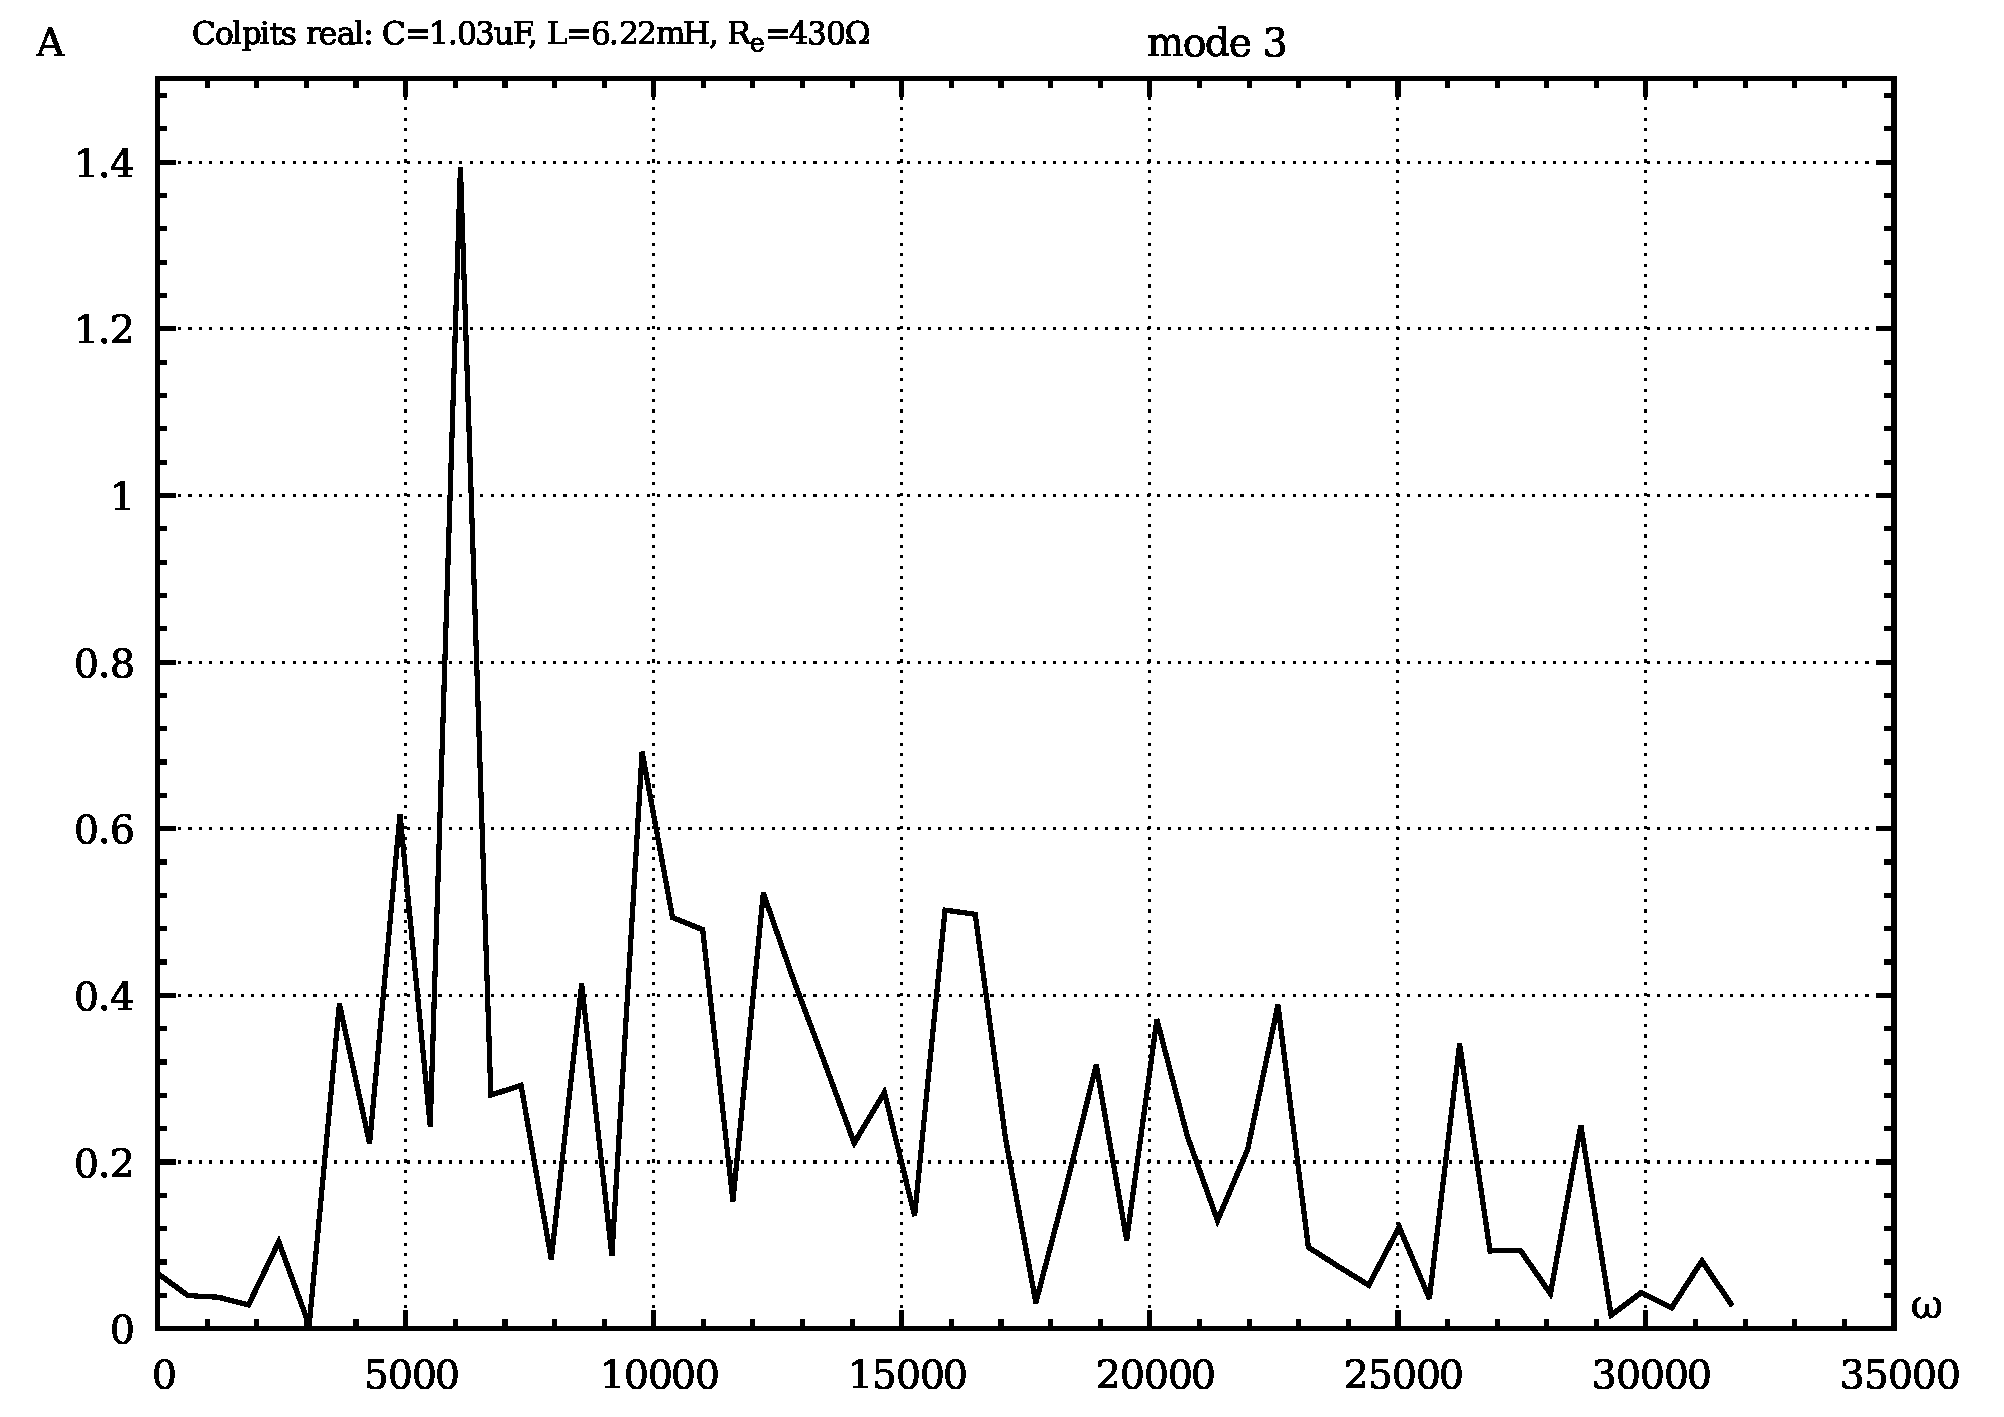
\includegraphics[width=0.32\textwidth]{p/cha/colp/colp_m3_f.png}
 }
  \caption{Спектры реальной системы Колпитца  для трёх режимов}
  \label{atu:f:colp_real_f}
\end{figure}

\begin{figure}[htb!]
 \centerline{
   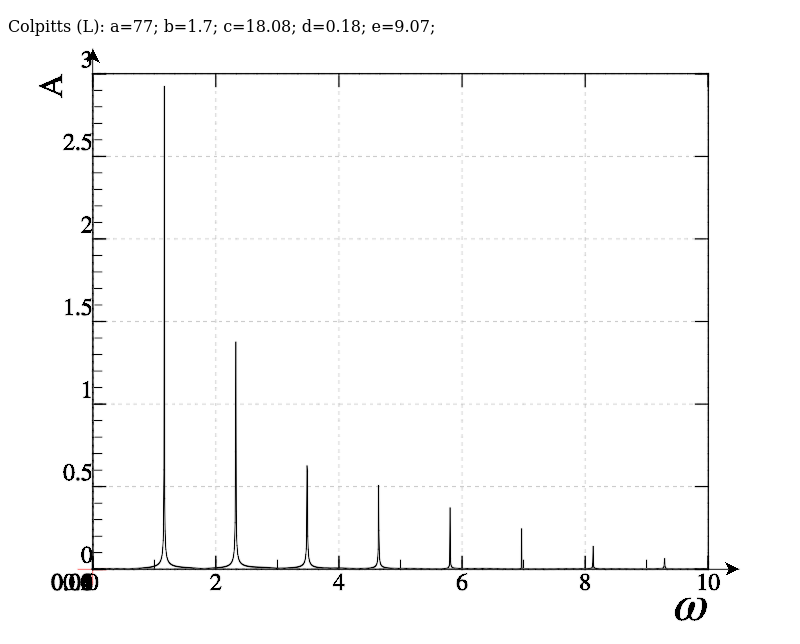
\includegraphics[width=0.32\textwidth]{p/cha/colp/colp_f-p_f_b=1x70.png}
   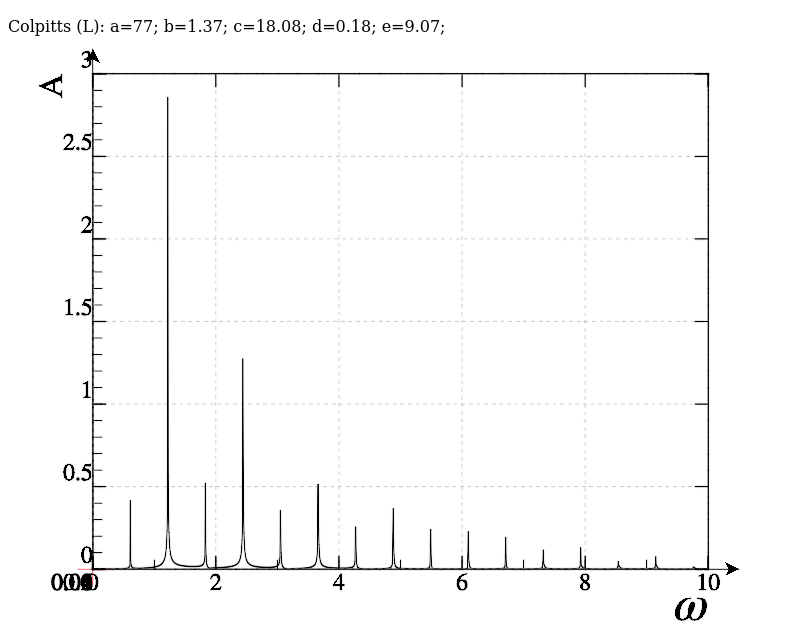
\includegraphics[width=0.32\textwidth]{p/cha/colp/colp_f-p_f_b=1x37.png}
   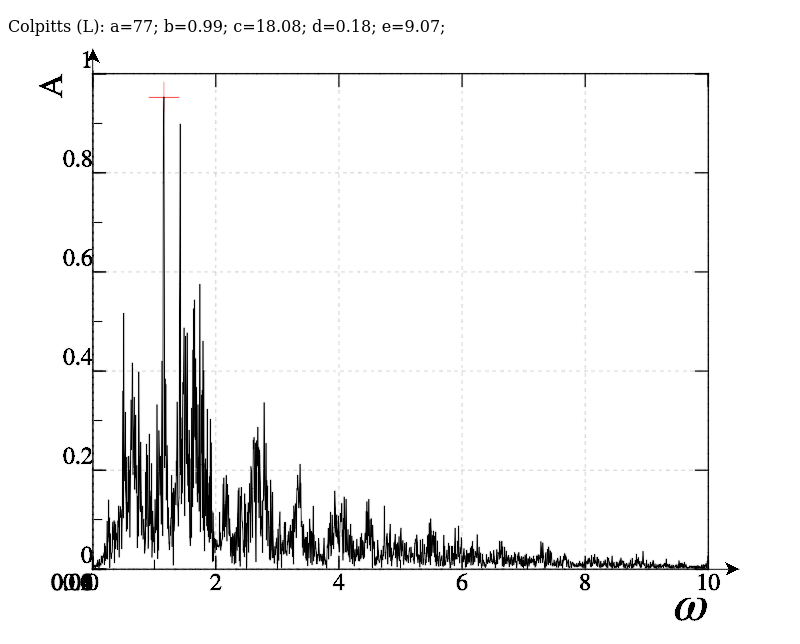
\includegraphics[width=0.32\textwidth]{p/cha/colp/colp_f-p_f_b=0x99.png}
 }
  \caption{Спектры модели (\ref{atu:eq:colp}) системы Колпитца для трёх режимов}
  \label{atu:f:colp_model_f}
\end{figure}

Сравнение результатов физического и численного моделирования позволяет сделать вывод
о качественном подобии поведения реальной системы и модели.
Тем не менее, величины параметра $b$, при которых получены
рассматриваемые режимы, совпадают весьма приближённо.
Для реальной системы значения параметра: $b = 1.06, \; 0.94, \; 0.90 $, в то время как
для модели: $b = 1.70, \; 1.34, \; 0.99 $.
Расхождение значений, скорее всего, связано с грубостью модельного представления (\ref{atu:eq:bjt_libear_model}) транзистора.
Вопрос применимости различных моделей биполярного транзистра в рамках рассмативаемой системы
требует дальнейшего исследования.
С другой стороны, ограниченный набор данных, получаемых с осциллографа Rigol DS1052E (8192 отсчёта) не позволяют
получить достаточно подробный спектр реальной системы.

Для определения критерия идентификации рассмотрим зависимости
$q_{*}(\mu) $, полученные путём моделирования
для системы Колпитца (рис.~\ref{atu:f:colp_q}).
При этом следует учесть, что наиболее просто измеряемыми величинами являются $x$ и $z$,
соответствующие напряжениям $V_1$ и $V_2$.
Первый набор зависимостей даёт два основных кандидата -- $q_{x^2}$ и $q_{z^2}$.
При этом первый из них показывает более равномерную зависимость.
В то же время, большинство из рассморенных зависимостей имею явно
выраженный гиперболический характер, особенно при малых значениях $b$.
Следовательно, в список кандидатов следует добавить $q_{x^{-2}} $ и $q_{z^{-2}}$.

\begin{figure}[htb!]
\centerline{
  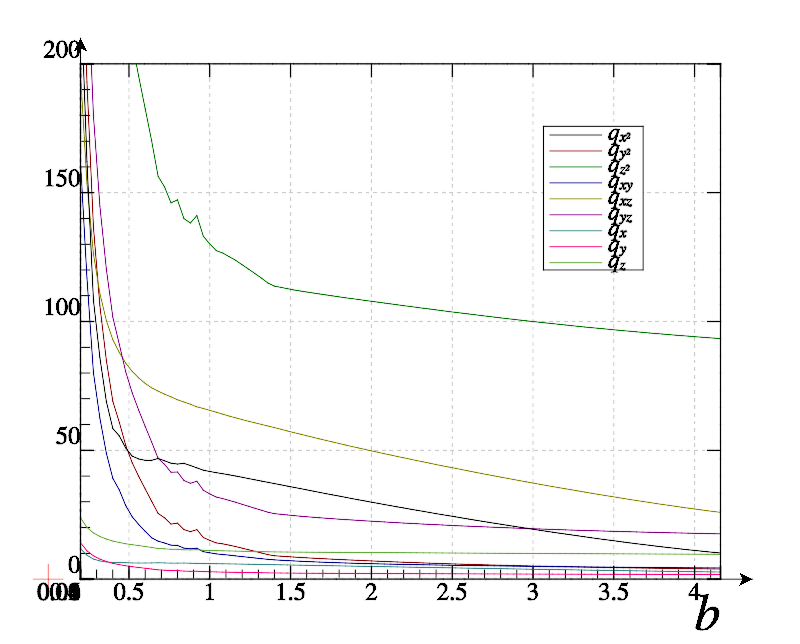
\includegraphics[width=0.49\textwidth]{p/cha/colp/colp_p-p_b_e.png}
  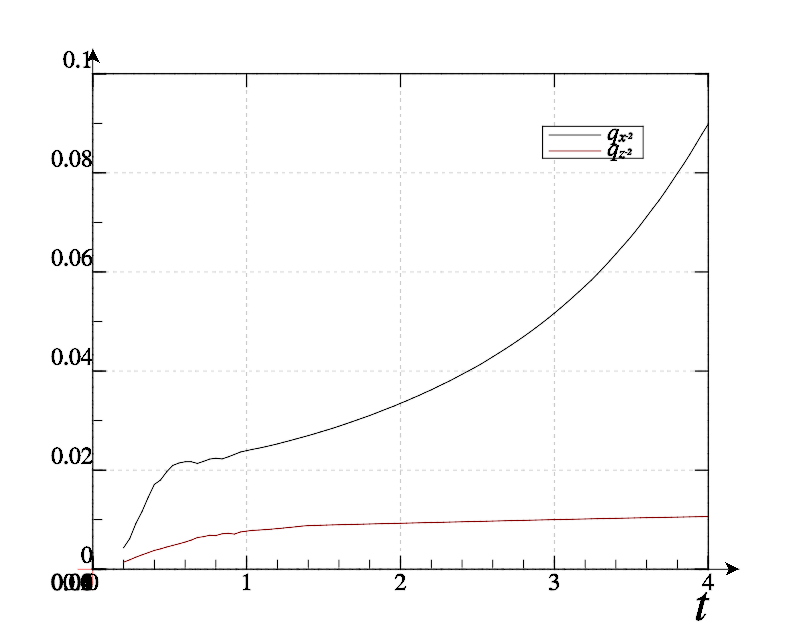
\includegraphics[width=0.49\textwidth]{p/cha/colp/colp_p-p_b_1ex2.png}
}
  \caption{Зависимости $q_{*}(b) $ для системы Колпитца (\ref{atu:eq:colp})}
\label{atu:f:colp_q}
\end{figure}

Из графиков очевидно, что
обратные зависимости не дают заметного выигрыша, поэтому выберем
величину $ q_{x^2}(b) $ в качестве критерия.

В качестве системы идентификации использовалась система с пятью поисковыми агентами и
двумя неподвижными моделями. Аналогично предыдущим системам,
для исследования динамических свойств системы идентификации
изменения параметра $b_o$ как:
%
\begin{equation}
 b_o(t) = p_0 + U_p \sign \sin( \omega_p t ),
  \label{atu:eq:colp_b_sign}
\end{equation}
%
\begin{equation}
 b_o(t) = p_0 + U_p \sin( \omega_p t ).
  \label{atu:eq:colp_b_sin}
\end{equation}

Динамика процессов идентификации для системы Колпитца представлена на рис.~\ref{atu:f:colp_id}.

\begin{figure}[htb!]
\centerline{
  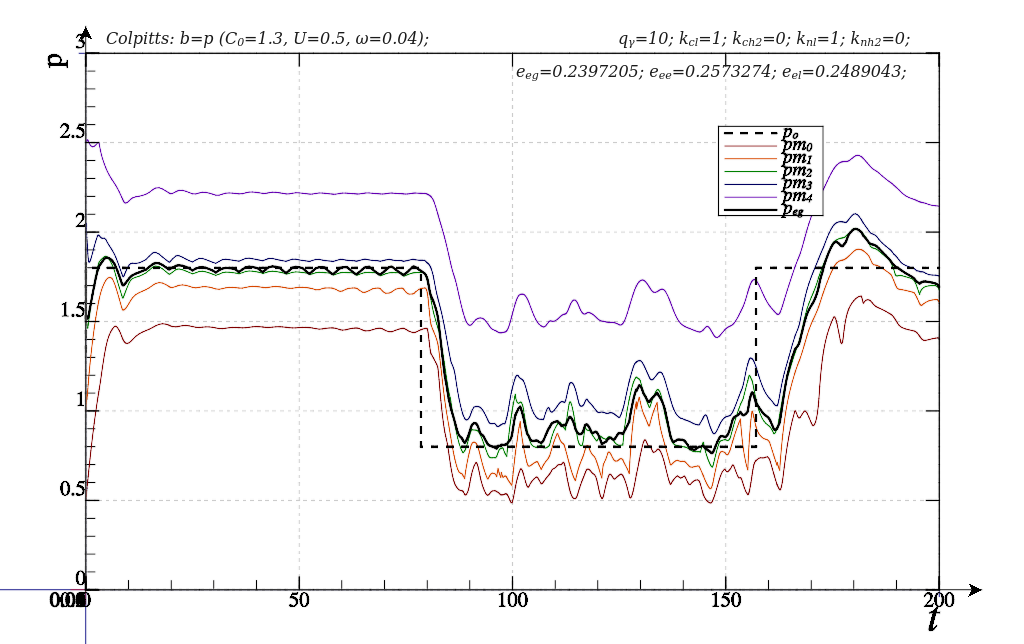
\includegraphics[width=0.49\textwidth]{p/cha/colp/colp_m5p-pl_n_sign.png}
  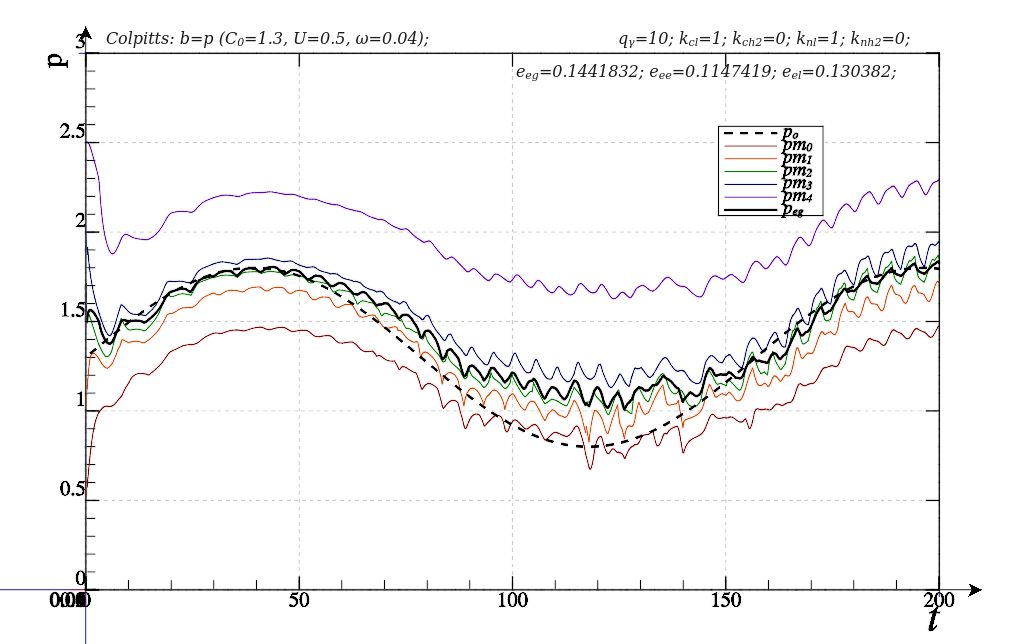
\includegraphics[width=0.49\textwidth]{p/cha/colp/colp_m5p-pl_n_sin.png}
}
\caption{Процесс идентификации параметра $b$ системы (\ref{atu:eq:colp})
  при условиях (\ref{atu:eq:colp_b_sign}) и (\ref{atu:eq:colp_b_sin})
}
\label{atu:f:colp_id}
\end{figure}

Зависимость среднеквадратических ошибок идентификации от величины $q_\gamma$ (рис.~\ref{atu:f:colp_e_qgamma})
даёт информацию о корректной настройке этого параметра системы идентификации.

\begin{figure}[htb!]
\centerline{
  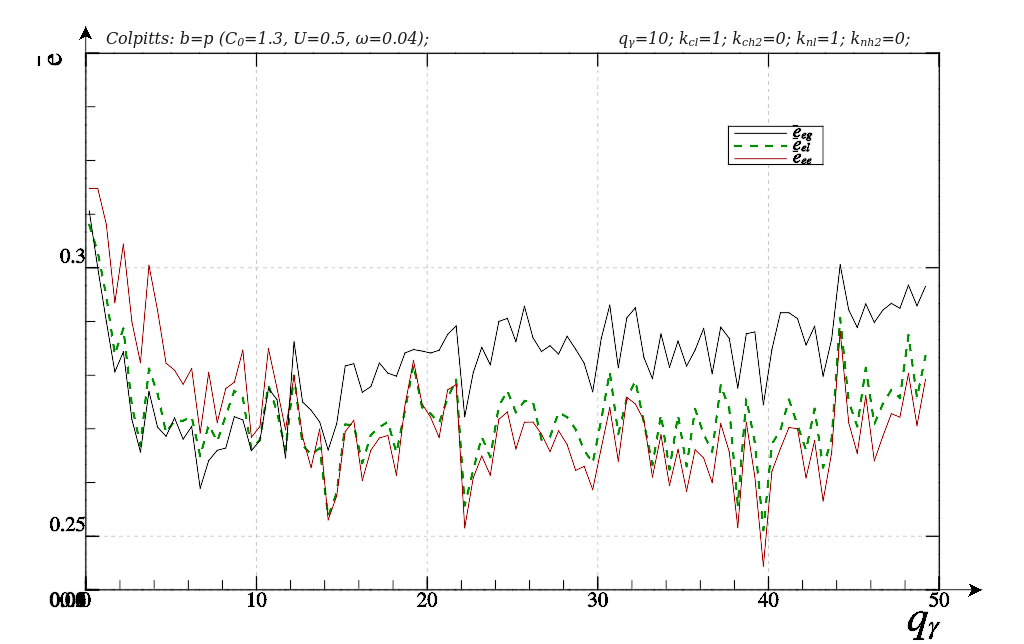
\includegraphics[width=0.49\textwidth]{p/cha/colp/colp_m5p-p_qg_e_sign.png}
  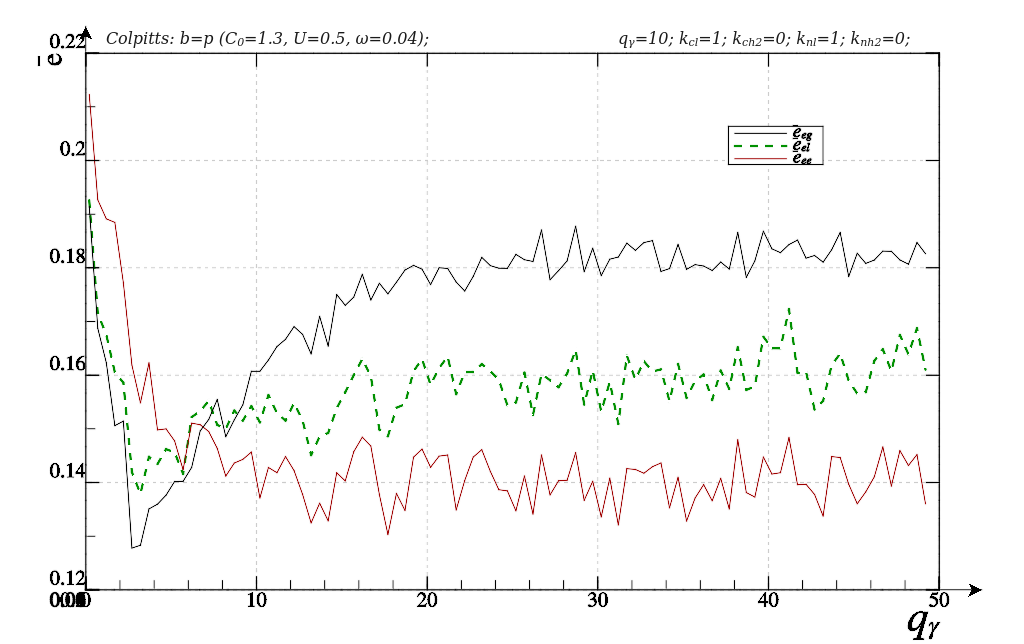
\includegraphics[width=0.49\textwidth]{p/cha/colp/colp_m5p-p_qg_e_sin.png}
}
  \caption{Зависимости  $\overline{e}(q_\gamma)$ для системы (\ref{atu:eq:colp})
  при условиях (\ref{atu:eq:colp_b_sign}) и (\ref{atu:eq:colp_b_sin})
}
\label{atu:f:colp_e_qgamma}
\end{figure}



Аналогично, зависимости $\overline{e_*}(a_q)$ (рис.~\ref{atu:f:colp_e_a_q})
позволяют корректно определить время усреденения.
При этом следует отметить, что
полученные результаты хорошо согласуются со спектрами системы.

\begin{figure}[htb!]
\centerline{
  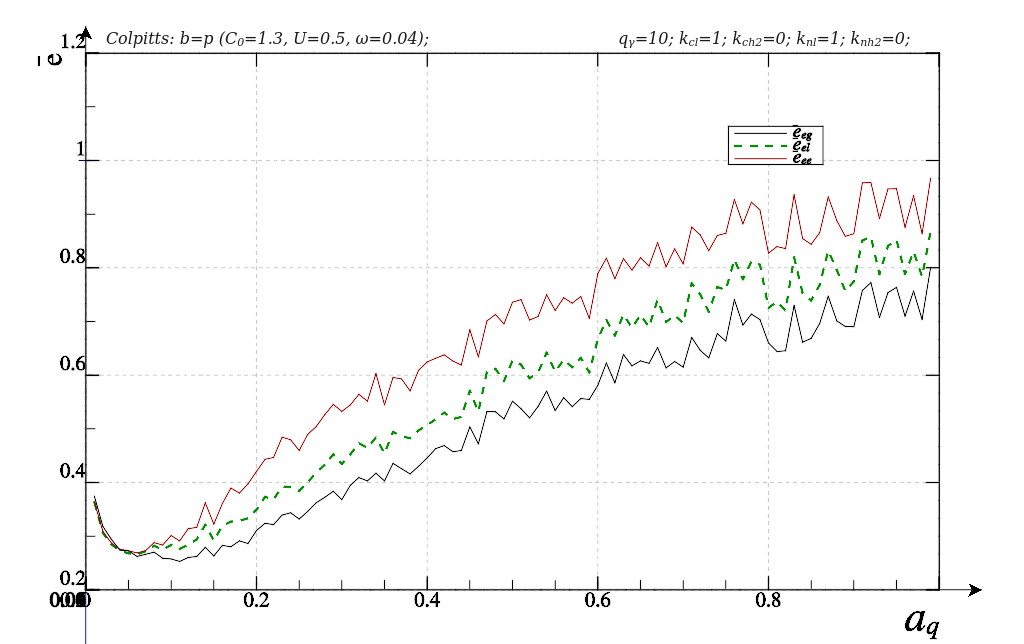
\includegraphics[width=0.49\textwidth]{p/cha/colp/colp_m5p-p_a_q_e_sign.png}
  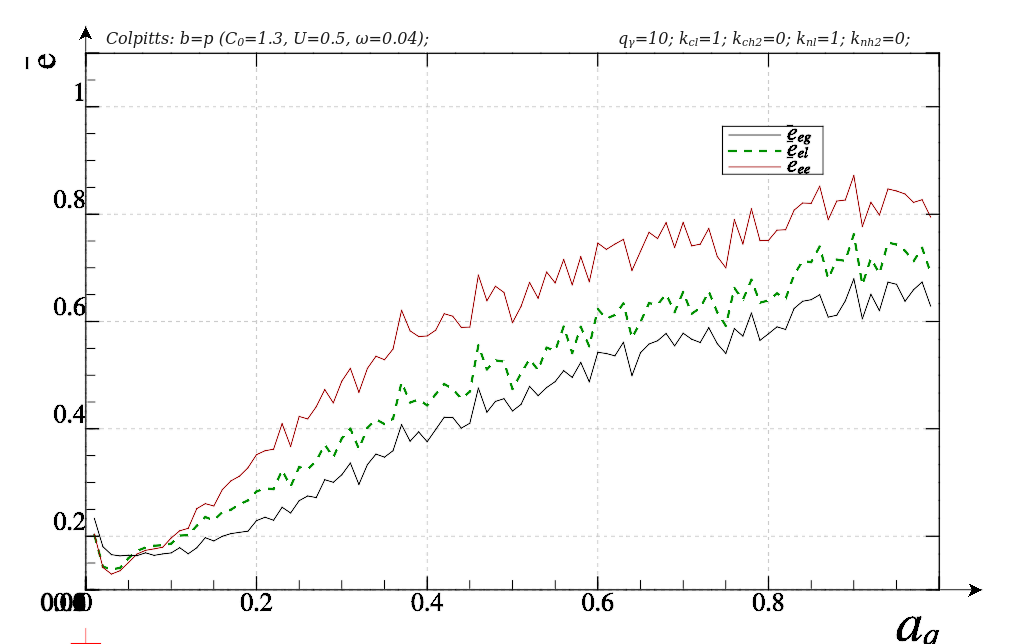
\includegraphics[width=0.49\textwidth]{p/cha/colp/colp_m5p-p_a_q_e_sin.png}
}
  \caption{Зависимости  $\overline{e}(a_q)$ для системы (\ref{atu:eq:colp})
  при условиях (\ref{atu:eq:colp_b_sign}) и (\ref{atu:eq:colp_b_sin})
}
\label{atu:f:colp_e_a_q}
\end{figure}

В целом синтез критерия идентификации и построение работоспособной системы идентификации для
системы генератора Колпитца не потребовало никаких специальных подходов и введения дополнительных
мер оценивания взаимосвязей параметров генератора.

